% !TeX root = Protokoll.tex
% !TeX root = ../../.global/latex/preamble.tex
\subsection{Magnetische Momente}
Ein Elektron im Atom besitzt zum einem den Bahndrehimpuls $\vec{l}$ und zum anderen
den, auch Eigendrehimpuls genannten, Spin $\vec{s}$.
Die Beträge dieser vektoriellen Größen werden bestimmt durch
\begin{align}
	|\vec{l}|=&\sqrt{l(l+1)}\hbar\\
	\nonumber &\text{und}\\
	|\vec{s}|=&\sqrt{s(s+1)}\hbar.
\end{align}
Dabei sind $l$ und $s$ die Drehimpuls- respektive Spinquantenzahl, sowie $\hbar$ das Plancksche Wirkungsquantum.
Aufgrund dieser Drehimpulse und der Ladung der Elektronen,
entstehten magnetische Momente $\vec{\mu_l}$ und $\vec{\mu_s}$.
Mithilfe des Bohrschen Magnetons
\begin{align}
	\mu_B:=-\frac{1}{2}e_0 \frac{\hbar}{m_0},
\end{align}
lassen sich diese Momente berechnen durch
\begin{align}
	\vec{\mu}_l=&-\mu_B\sqrt{l(l+1)}\vec{e}_l\\
	\nonumber &\text{und}\\
	\vec{\mu}_s=&-g_s\,\mu_B\sqrt{s(s+1)}\vec{e}_s.
\end{align}
Hier ist $e_0$ die Elementarladung und $m_0$ die Elektronmasse.
Weiter wird für $\vec{\mu}_s$ der Landé-Faktor eingeführt, der die Stärke der Kopplung
des Spins ans magnetische Moment beschreibt.

Für Atome mit mehr als ein Elektron gibt es verschiedene Arten,
wie der Bahndrehimpulse und der Spin wechselwirken können.
Grundlegend können zwei  Grenzfälle unterschieden werden.
Zum einen für Atome mit niedriger und zum anderen für Atome mit hoher Kernladungszahl.
Bei Atomen mit niedriger Kernladungszahl, ist die Wechselwirkung unter den Drehimpulsen $l_{i}$
der einzelnen Elektronen groß.
Deshalb lässt sich ein Gesamtdrehimpuls der Elektronenhülle definieren als
\begin{align}
	\vec{L}:=\sum_i \vec{l}_i\, \text{ mit }\, |\vec{L}|=\sqrt{L(L+1)}\hbar.
\end{align}
Weil der Drehimpuls abgeschlossener Schalen immer Null ist,
reicht es aus über die Drehimpulse der der nicht abgeschlossenen Schalen zu summieren.
Es treten dabei nur Gesamtdrehimpulse auf, deren Quantenzahl $L$ ganzzahlig ist.
Dabei wird der Wert der Quantenzahl $L$ mit den Buchstaben S, P, D oder F
(für die Werte 0, 1, 2 und 3) angegeben.\\
Zu dem Gesamtbahndrehimpuls lässt sich ein magnetisches Moment $\vec{\mu}_L$ mit dem Betrag
\begin{align}
	|\vec{\mu}_L|=\mu_B\sqrt{L(L+1}).
\end{align}
aufstellen.
Analog zu $\vec{L}$ lässt sich weiter ein Gesamtspin der Elektronenhülle
\begin{align}
	\vec{S}=\sum_is_i \text{ mit } |\vec{S}|=\sqrt{S(S+1)}\hbar
\end{align}
definieren.
Für die Gesamtspinquantenzahl gilt $S=\frac{N}{2},\ \frac{N}{2}-1 ,\ \dots,\ \frac{1}{2},\ 0$,
wobei $N$ die Anzahl der Elektronen der nicht abgeschlossenen Schale ist.
Der Betrag des magnetische Moments, das durch den Gesamtspin hervorgerufen wird, lässt sich mit
\begin{align}
	|\vec{\mu}_S|=g_S\ \mu_B\sqrt{S(S+1)}
\end{align}
berechnen.
Bei nicht zu großen externen Magnetfeldern lässt sich der Gesamtdrehimpuls
\begin{align}
	\vec{J}=\vec{L}+\vec{S} \ \text{ mit }\ |\vec{J}|=\sqrt{J(J+1)}\hbar.
\end{align}
bestimmen.
Ein Energie Niveau kann mithilfe von
\begin{align}
	{}^M\mathcal{L}_J
\end{align}
beschrieben werden.
Darin bezeichnet $M=2S+1$ und $\mathcal{L}\in\{S(L=0), P(L=1), D(L=2), F(L=3)\}$
bezeichnet die Quantenzahlen des Bahndrehimpulses $L$.
Diese Art der Kopplung wird LS-Kopplung genannt.\\
Der Zweite Fall, der bei großer Kernladungszahl auftritt, wird j-j-Kopplung genannt.
Hier koppelt der Spin und der Bahndrehimpuls eines Elektrons stark,
gegenüber der Kopplung mit den anderen Elektronen.
Dadurch addieren sich der Spin und der Bahndrehimpuls zum Gesamtdrehimpuls des Elektrons, so dass
\begin{align}
	\vec{j}_i=\vec{l}_i+\vec{s}_i
\end{align}
gilt.
Dann lässt sich der Gesamtdrehimpuls der Elektronenhülle schreiben als
\begin{align}
	\vec{J}=\sum_i\vec{j}_i,
\end{align}
allerdings kann weder ein Gesamtbahndrehimpulse $\vec{L}$
noch ein Gesamtspins $\vec{S}$ definiert werden.
Für Atome mit einer mittel hohen Ladungszahl besteht zwischen diesen beiden Grenzfällen ein fließender Übergang.

Zu dem Gesamtdrehimpuls $\vec{J}$ lässt sich ein magnetisches Moment berechnen als
\begin{align}
	\vec{\mu}_J&=\mu_Bg_J\sqrt{J(J+1)},
\end{align}
wobei
\begin{align}
		g_J:=&\frac{3J(J+1)+S(S+1)-L(L+1)}{2J(J+1)}
\end{align}
gilt.
Dabei wird $g_J$ als Landé-Faktor des entsprechenden Atoms bezeichnet.
\subsection{Energieaufspaltung und Übergänge}
\begin{figure}[h!]
	\centering
	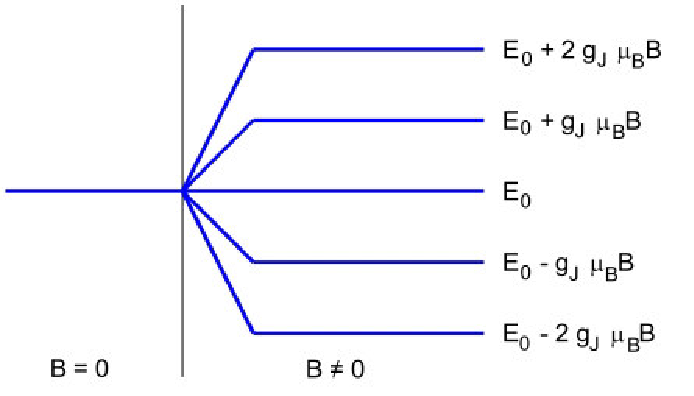
\includegraphics[width=0.6\textwidth]{../Grafiken/fig_theo_Aufspaltung.pdf}
	\caption{Aufspaltung eines Energieniveaus von einem Atom mit $J=2$. \cite{V27}}\label{fig:Theo_Aufspaltung}
\end{figure}
\noindent
Wird an einem Atom mit Gesamtdrehimpuls $\vec{J}$ ein homogenes Magnetfeld
$\vec{B}$ angelegt, so ist die resultierende Energie
\begin{align}
	E_\text{mag}= -\vec{\mu}_J\cdot\vec{B}=mg_J\mu_BB,
\end{align}
wobei $m$ die ganzzahlige Orientierungsquantenzahl ist, für die gilt $-J\le m\le J$.
Dies gilt, da nur bestimmte Winkel zwischen dem Magnetfeld und dem magnetischen Moment auftreten,
sodass die $z$-Komponente ein ganzzahliges Vielfaches von $g_J\mu_B$ ist.
Es tritt demnach eine Aufspaltung in $2J+1$ Niveaus auf, dies ist anhand des
Beispiels $J=2$ in \cref{fig:Theo_Aufspaltung} dargestellt.

Die Übergänge der Energieniveaus wird mithilfe der zeitabhängigen Schrödingergleichung
\begin{align}
	\frac{\hbar^2}{2m}\Delta \psi(\vec{r},t)+U\psi(\vec{r},t)-i\hbar\frac{\partial \psi(\vec{r},t)}{\partial t}=0
\end{align}
beschrieben.
Dabei sollen Lösungen $\psi$ gefunden werden die den Übergang zwischen zwei Energieniveaus
$\alpha$ und $\beta$ beschreiben. Aus diesen ergibt sich eine Oszillation
mit der Frequenz
\begin{align}
	\nu_{\alpha\beta}:=\frac{E_\alpha-E_\beta}{h}
\end{align}
zwischen den beiden Niveaus.
Daraus lässt sich erkennen, dass sich das Elektron als Dipol beschreiben lässt.
Das Dipolmoment in $x$-Richtung kann mithilfe von
\begin{align}
	D_x=-e_0\text{const}\real\left( \underbrace{\int x\psi^*_\beta\psi_\alpha dV}_{X_{\alpha\beta}}\exp(2\pi i\nu_{\alpha\beta}t) \right),
\end{align}
ausgedrückt werden.
Analog können die Komponenten für die $y$ und $z$-Richtung aufgestellt werden.
Die dabei auftretenden Integrale der Form
\begin{empheq}{equation}
	X_{\alpha\beta} = \int_{}^{} x \psi^{*}_{\alpha} \psi_{\beta} \dif V
\end{empheq}
(analog für $y$ und $z$) werden als Matrixelemente bezeichnet.
Es kann gezeigt werden, dass die Intensität der vom Dipol emittierten Strahlung
mit diesen Matrixelementen zusammenhängt.
Die Matrixelemente $Z_{\alpha\beta}$, $X_{\alpha\beta}\pm i Y_{\alpha\beta}$ verschwinden, es sei den es gilt
\begin{align}
	\Delta m = m_\alpha-m_\beta = 0,\pm 1
\end{align}
Aus der Konstruktion der Matrixelemente kann geschlossen werden, dass bei
$\Delta m=0$ ($Z_{\alpha\beta}\neq=0,\ X_{\alpha\beta}\pm i Y_{\alpha\beta}=0$)
der Dipol entlang der Magnetfeldachse schwingt und somit parallel zum Magnetfeld
linear-polarisiertes Licht abstrahlt, diese Strahlungsart wird mit einem $\pi$ gekennzeichnet.
Für $\Delta m =\pm 1$ gilt $Z_{\alpha\beta}=0$ und
$\ X_{\alpha\beta}\pm i Y_{\alpha\beta}\not=0$, daraus lässt sich schließen,
dass entweder links oder rechts (um die Magnetfeldachse) zirkular-polarisierte Strahlung emittiert wird.
Diese wird als $\sigma$-Emission bezeichnet.

Die obigen Überlegungen gelten zunächst nur für den Fall $S=0$,
dieser Spezialfall wird als normaler Zeeman-Effekt bezeichnet.
Bei Übergängen mit $S=0$ gilt $g_J=1$, wodurch die Energieunterschiede $\Delta E$ zwischen
den aufgespaltenen Niveaus mit
\begin{empheq}{equation}
	\Delta E = \Delta m \mu_{B} B
\end{empheq}
unabhängig von den Quantenzahlen $L$ und $J$ gleich groß sind.

Bei dem anormalen Zeeman-Effekt verschwindet die Spinquantenzahl nicht.
Hier bei gelten die selben Auswahlregeln $\Delta m=0,\pm 1$ für Übergänge.
Allerdings ist damit nicht mehr $g_J=1$ gegeben, deshalb ergibt sich die Energie der Spektrallinie zu
\begin{align}
	E=\underbrace{(m_ig_{J_i}-m_jg_{J_j)}}_{g_{ij}}\mu_BB+E_0=g_{ij}\mu_BB+E_0.
	\label{eq:anormaler_zeemann_energie}
\end{align}
Darin ist $g_{ij}$ der Landé-Faktor des Übergangs.

\subsection{Übergänge der Cd-Lampe}
In diesem Versuch werden die Übergänge von Cadmium untersucht, indem
die Aufspaltung von zwei Spekrallinien einer Cd-Lampe aufgenommen werden.
%Deshalb ist es von Interesse diese Übergänge genauer zu untersuchen.
%Hier werden zwei Spektrallinien untersucht.
Zum einen wird die rote Spektrallinie mit einer Wellenlänge von $\SI{643,8}{\nano\meter}$, die durch den Übergang
${}^1P_1\leftrightarrow{}^1D_2$ hervorgerufen wird untersucht.
Zum anderen wird die blaue Spektrallinie mit einer Wellenlänge von $\SI{480}{\nano\meter}$ betrachtet,
die durch den Übergang ${}^1S_1\leftrightarrow{}^3P_1$ ausgelöst wird.
Die Termschemata sind in \cref{fig:termschema_rot} und \cref{fig:termschema_blau} dargestellt.
Die zugehörigen Landé-Faktoren werden in \cref{tab:Lande_rot} und \cref{tab:Lande_blau} berechnet.
Dabei entspricht die rote Spektrallinie dem normalen Zeeman-Effekt und die blaue dem anormalen Zeeman-Effekt.
%\subsection{Vorbereitungaufgaben}

\FloatBarrier
\begin{figure}[!h]
\centering
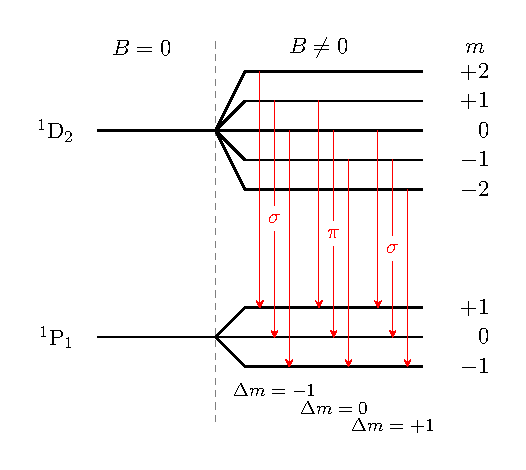
\includegraphics[scale=1.15]{../Grafiken/termschema_rot.pdf}
\caption{Hier ist das Termschema der roten Spektrallinie einer Cd-Lampe dargestellt\label{fig:termschema_rot}}
\end{figure}
\FloatBarrier
\FloatBarrier
\begin{figure}[!h]
\centering
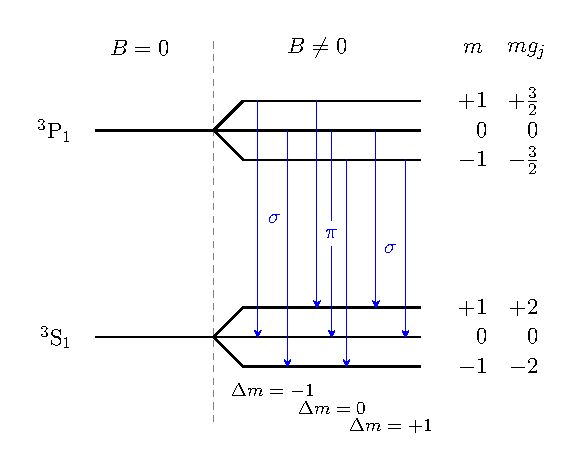
\includegraphics[scale=1.25]{../Grafiken/termschema_blau.pdf}
\caption{\label{fig:termschema_blau}}
\end{figure}
\FloatBarrier

\begin{table}
	\centering
	\begin{tabular}{cccccc}
		\toprule
		Übergang & $m_1$  & $g_{1}$ & $m_2$ & $ g_2$ & $g_{12}$\\
		\midrule
		& \multicolumn{2}{c}{${}^1P_1$}  & \multicolumn{2}{c}{${}^1D_2$} \\
		\midrule
		& 2 & 1 & 1 & 1 & 1\\
		$\sigma$& 1 & 1 & 0 & 1 & 1\\
		& 0 & 1 & -1 & 1 & 1\\
		\midrule
		& 1 & 1 & 1 & 1 & 0\\
		$\pi$ & 0 & 1 & 0 & 1 & 0\\
		& -1 & 1 & -1 & 1 & 0\\
		\midrule
		& 0 & 1 & 1 & 1 & -1\\
		$\sigma$ & -1 & 1 & 0 & 1 & -1\\
		& -2 & 1 & -1 & 1 & -1\\\bottomrule
	\end{tabular}
	\caption{Hier sind die Landé-Faktoren der roten Spektrallinie aufgeführt.}
	\label{tab:Lande_rot}
\end{table}
\begin{table}
	\centering
	\begin{tabular}{cccccc}
		\toprule
		Übergang & $m_1$  & $g_{1}$ & $m_2$ & $ g_2$ & $g_{12}$\\
		\midrule
		& \multicolumn{2}{c}{${}^3S_1$}  & \multicolumn{2}{c}{${}^3P_2$} \\
		\midrule
		$\sigma$ & +1 & 2 & 0 & $\frac{3}{2}$& 2\\
		& 0 & 2 & -1 & $\frac{3}{2}$ & $\frac{3}{2}$\\
		\midrule
		& +1 & 2 & +1 & $\frac{3}{2}$ & $\frac{1}{2}$\\
		$\pi$ & 2 & 2 & 0 & $\frac{3}{2}$ & 0 \\
		& -1 & 2 & -1 & $\frac{3}{2}$ & -$\frac{1}{2}$\\
		\midrule
		& 0 & 2 & 1 & $\frac{3}{2}$ & -$\frac{3}{2}$\\
		$\sigma$ & -1 & 2 & 0 & $\frac{3}{2}$& -2\\
		\bottomrule
	\end{tabular}
	\caption{Hier sind die Landé-Faktoren der blauen Spektrallinie aufgeführt.}
	\label{tab:Lande_blau}
\end{table}
